\documentclass[xcolor=dvipsnames]{beamer} % dvipsnames gives more built-in colors
\usepackage[utf8]{inputenc}
\usepackage[english]{babel}
\usepackage{xcolor}
\usepackage{listings}
\usepackage{caption}

\usetheme{Madrid}
\useoutertheme{miniframes} % Alternatively: miniframes, infolines, split
\useinnertheme{circles}

\definecolor{UBCblue}{rgb}{0.04706, 0.13725, 0.26667} % UBC Blue (primary)


\lstset{ %
  backgroundcolor=\color{white}, 
  basicstyle=\footnotesize,       
  breakatwhitespace=false,        
  breaklines=true,                 
  captionpos=b,                    
  commentstyle=\color{green},   
  escapeinside={\%*}{*)},        
  extendedchars=true,              
  frame=single,                  
  keywordstyle=\color{blue},       
  language=Prolog,                
  numbers=left,                    
  numbersep=5pt,                   
  numberstyle=\tiny\color{gray},
  rulecolor=\color{black},        
  showspaces=false,               
  showstringspaces=false,          
  showtabs=false,                  
  stepnumber=2,                    
  stringstyle=\color{BrickRed},   
  tabsize=2,                      
  title=\lstname,                  
  morekeywords={not,\},\{,preconditions,effects },            
  deletekeywords={time}            
}

\usecolortheme[named=UBCblue]{structure}
%\usecolortheme[named=Mahogany]{structure} % Sample dvipsnames color

\title[VirtShell]{\textbf{VirtShell} \\ Framework para aprovisionamiento de soluciones virtuales}
\date{\today}
\titlegraphic{
\includegraphics[width=1.0cm]{logo_univalle.pdf}}                                                                                                           \author[CALlanoR]{\textbf{Carlos Alberto Llano R.}}
\institute[www.univalle.edu.co]{Escuela de Ingeniería de Sistemas y Computación \\ Maestría en Ingeniería con énfasis en Ingeniería de Sistemas}

\begin{document}

\frame{\titlepage}

\frame{\frametitle{Contents}\tableofcontents}

\logo{\hspace*{0.6\textwidth}
\includegraphics[width=0.6cm]{logo_univalle}\hspace*{0.3cm}}

\section{Flujo de aprovisionamiento}
\frame{ \frametitle{Flujo}
\begin{figure}
	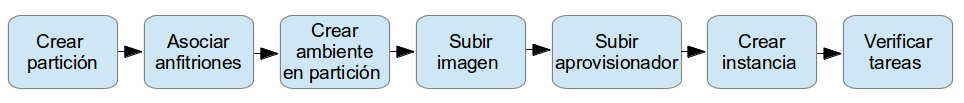
\includegraphics[width = 0.9\textwidth]{../figures/general_workflow_provisioning}
\end{figure}

}

\frame{ \frametitle{Particiones y Anfitriones}
\begin{figure}
	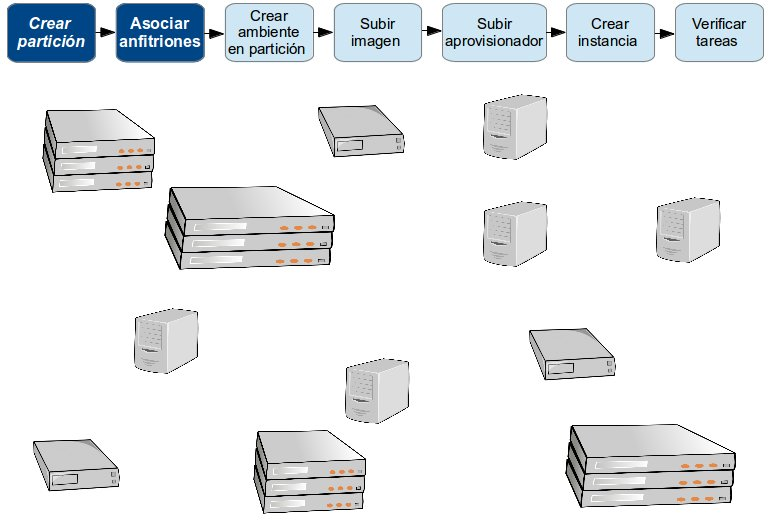
\includegraphics[width = 0.8\textwidth]{../figures/partitions_and_hosts}
\end{figure}
}


\frame{ \frametitle{Particiones y Anfitriones}
\begin{figure}
	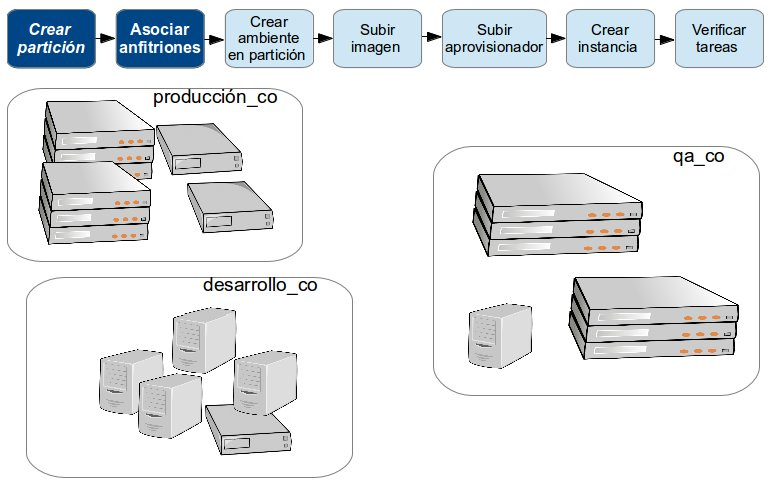
\includegraphics[width = 0.8\textwidth]{../figures/partitions_and_hosts2}
\end{figure}
}

\begin{frame}[fragile]
\frametitle{Particiones y Anfitriones (Ejemplo)}
\begin{lstlisting}[language=Bash,basicstyle=\ttfamily\scriptsize,keywordstyle=\color{blue}]
curl -X POST http://virtshellsrv:80/partitions/ 
    -d "{\"name\":\"development_co\",
         \"description\":\"Collection of servers oriented to development team in Colombia.\"}" 
    -H "accept:application/json" | jq .
\end{lstlisting}
\end{frame}


\frame{ \frametitle{Ambientes de trabajo}
\begin{figure}
	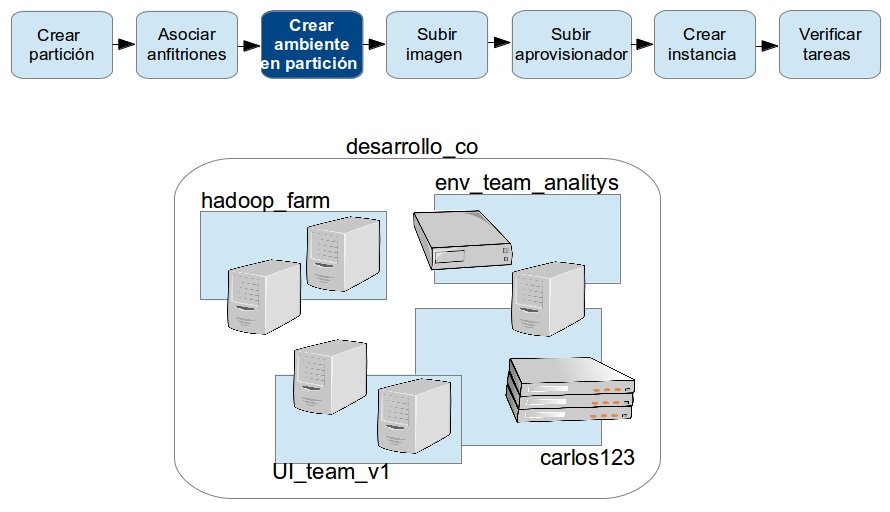
\includegraphics[width = 0.8\textwidth]{../figures/enviroments}
\end{figure}
}

\begin{frame}[fragile]
\frametitle{Ambientes de trabajo (Ejemplo)}
\begin{lstlisting}[language=Bash,basicstyle=\ttfamily\scriptsize,keywordstyle=\color{blue}]
curl -X POST http://virtshellsrv:80/enviroments/ 
    -d "{\"name\":\"development\",
         \"description\":\"Development enviroment\", 
         \"partition\": \"development_co\", 
         \"users\": [{\"login\": \"development_user\"}, 
                     {\"login\": \"guest\"}]}" 
    -H "accept:application/json" | jq .
\end{lstlisting}
\end{frame}

\frame{ \frametitle{Imagenes}
}

\frame{ \frametitle{Aprovisionadores}
}

\frame{ \frametitle{Creación de instancias}
}

\frame{ \frametitle{Chequeo de tareas}
}

\section{Arquitectura}
\frame{ \frametitle{Framework}
\begin{figure}
	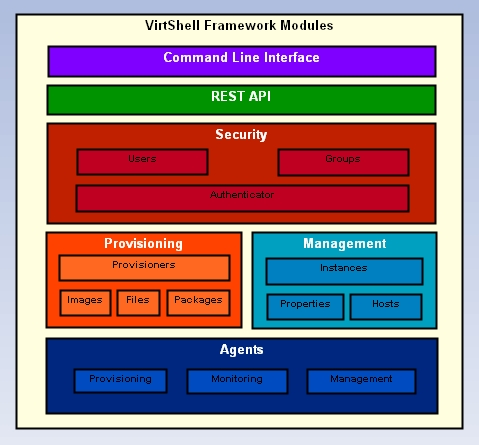
\includegraphics[width = 0.5\textwidth]{../../architecture/v1/diagrams/framework}
\end{figure}
}

\frame{ \frametitle{Vista de componentes}
}

\frame{ \frametitle{Vista de deployment}
}

\section{Pruebas y Resultados}
\frame{ \frametitle{Pruebas y Resultados}
}

\section{Conclusiones}
\frame{ \frametitle{Conclusiones}
}

\section{Recomendaciones}
\frame{ \frametitle{Recomendaciones}
}

\frame{ \frametitle{Preguntas?}
\begin{figure}
	
\includegraphics[width = 0.2\textwidth]{../figures/preguntas}
\end{figure}
}

\end{document}